\documentclass[]{article}
\newcommand{\FileDepth}{../../..}
\usepackage[letterpaper, landscape, margin=0.5cm]{geometry}
\usepackage[T1]{fontenc}
\usepackage{textcomp}%Not strictly necessary, but gives \textmu command for "micro."
\usepackage{fancyhdr}
\usepackage{amsmath}
\usepackage{amssymb}
\usepackage{graphicx}
\usepackage{xcolor}
\usepackage{tikz}
\usetikzlibrary{calc}
\usepackage[shortlabels]{enumitem}
\usepackage{multicol}
\usepackage{vwcol}
\usepackage{hyperref}
\usepackage{wrapfig}
%opening
\newcommand{\SecType}{S}
\newcommand{\Week}{7}
\title{PH 211 Studio \Week}
\author{Benjamin Bauml}
\date{Summer 2024}

\newcommand{\Purpose}{4}
\newcommand{\DefOnly}{0}

% Version 2024-06-14
% Changes
% 2024-02-21 Added xstring package to enable smooth implementation of new \ModePage command.
% 2024-04-27 Set up to split activities and formatting aspects into separate files. Removed dependence on xcomment. Added an automatic counter to number the activities in a problem set.
% 2024-05-19 Revised old format for \TeachingTips command, which did not support \DefOnly.
% 2024-06-14 Added Repurpose environment to allow mixing of different purpose levels in the same document.
\usepackage{tcolorbox}
\usepackage{xstring}
% You will want the following four lines in your document (the last two uncommented):
% For Assignment, leave Purpose as 1. For Worksheet, set to 2. For Student Solution, set to 3. For Teacher Solution, set to 4.
% If you want keep the pieces from being called manually, set DefOnly to 0.
%\newcommand{\Purpose}{4}
%\newcommand{\DefOnly}{1}
\newcommand{\Exclusion}{0}
\newcommand{\PageTurn}{0}
\newcommand{\GrayProb}{0}
\newcommand{\Tipsy}{0}

% Assignment
\if\Purpose1
\renewcommand{\Exclusion}{1}
\fi
% Worksheet
\if\Purpose2
\renewcommand{\Exclusion}{1}
\renewcommand{\PageTurn}{1}
\fi
% Student Solution
\if\Purpose3
\renewcommand{\PageTurn}{1}
\renewcommand{\GrayProb}{1}
\fi
% Teaching Copy
\if\Purpose4
\renewcommand{\PageTurn}{1}
\renewcommand{\GrayProb}{1}
\renewcommand{\Tipsy}{1}
\fi

\newenvironment{Repurpose}[1]{
\renewcommand{\Purpose}{#1}
\renewcommand{\Exclusion}{0}
\renewcommand{\PageTurn}{0}
\renewcommand{\GrayProb}{0}
\renewcommand{\Tipsy}{0}
% Assignment
\if\Purpose1
\renewcommand{\Exclusion}{1}
\fi
% Worksheet
\if\Purpose2
\renewcommand{\Exclusion}{1}
\renewcommand{\PageTurn}{1}
\fi
% Student Solution
\if\Purpose3
\renewcommand{\PageTurn}{1}
\renewcommand{\GrayProb}{1}
\fi
% Teaching Copy
\if\Purpose4
\renewcommand{\PageTurn}{1}
\renewcommand{\GrayProb}{1}
\renewcommand{\Tipsy}{1}
\fi
}{}

\def \NewQ {0}
\def \PForce {0}
\newcommand{\MaybePage}[1]{
	\def \PForce {#1}
	\if\PForce1
	\newpage
	\else
	\if\NewQ0
	\gdef \NewQ {\PageTurn}
	\else
	\newpage
	\fi
	\fi
}

\newcommand{\ModePage}[1]{
	\IfSubStr{#1}{\Purpose}{\newpage}{}
}

\newcounter{ActNumber}
\setcounter{ActNumber}{0}

\newcommand{\Problem}[4][0]{%The first argument is optional, and if it is set to 1, the \newpage will be forced. The second argument is the name of the activity, the third is the command the activity is stored as, and the fourth is the actual problem statement.
\newcommand{#3}{
\MaybePage{#1}
\addtocounter{ActNumber}{1}
\section*{\SecType\Week-\theActNumber: #2}
\if\GrayProb1
\begin{tcolorbox}[colback=lightgray,colframe=lightgray,sharp corners,boxsep=1pt,left=0pt,right=0pt,top=0pt,bottom=0pt,after skip=2pt]
\else
\begin{tcolorbox}[colback=white,colframe=white,sharp corners,boxsep=1pt,left=0pt,right=0pt,top=0pt,bottom=0pt,after skip=2pt]
\fi
#4
\end{tcolorbox}\noindent
}
\if\DefOnly0
\else
#3
\fi
}
	
\newcommand{\ProblemSub}[3][0]{%The first argument is optional, and if a string of numbers is entered into it, it will force a \newpage in any \Purpose that shows up in the string. For example, "13" would lead to the newpage being forced in modes 1 and 3. The second is the command the activity is stored as, and the third is the actual problem statement.
\newcommand{#2}{
\ModePage{#1}
\if\GrayProb1
\begin{tcolorbox}[colback=lightgray,colframe=lightgray,sharp corners,boxsep=1pt,left=0pt,right=0pt,top=0pt,bottom=0pt,after skip=2pt]
\else
\begin{tcolorbox}[colback=white,colframe=white,sharp corners,boxsep=1pt,left=0pt,right=0pt,top=0pt,bottom=0pt,after skip=2pt]
\fi
#3
\end{tcolorbox}\noindent
}
\if\DefOnly0
\else
#2
\fi
}
		
\newcommand{\Solution}[2]{%The first argument is the command the solution is stored as, and the second is the actual solution.
\newcommand{#1}{
\if\Exclusion0
#2
\fi
}
\if\DefOnly0
\else
#1
\fi
}
		
\newcommand{\ProblemFig}[2]{%The first argument is the command the figure is stored as, and the second is the actual figure.
\newcommand{#1}{
\begin{figure}[h]
#2
\end{figure}
}
\if\DefOnly0
\else
#1
\fi
}

\newcommand{\TeachingTips}[2]{%The first argument is the command the tip is stored as, and the second is the actual tip.
\newcommand{#1}{
\if\Tipsy1
\begin{tcolorbox}[colback=lightgray,colframe=black]
#2
\end{tcolorbox}
\fi
}
\if\DefOnly0
\else
#1
\fi
}
\usepackage[absolute]{textpos}
% This package relies on Assignment Format 2024-06-14 or later to work. It is recommended that the Purpose and DefOnly commands be given as such:
%\newcommand{\Purpose}{4}
%\newcommand{\DefOnly}{0}
% Activities need to be entered outside of the TeacherMargin and PresentSpace environments, otherwise they will be defined only locally. They can even go in the preamble.
\newenvironment{TeacherMargin}{\begin{textblock*}{10.8cm}(0.5cm,0.5cm)
\small}{\end{textblock*}
\hspace{0.1cm}}
\newenvironment{PresentSpace}{\begin{textblock*}{0.3cm}(26.85cm,9.35cm)
--
\end{textblock*}
\begin{textblock*}{0.3cm}(26.85cm,18.7cm)
--
\end{textblock*}
\begin{textblock*}{0.3cm}(26.85cm,12.24cm)
	--
\end{textblock*}
\begin{textblock*}{15.6cm}(11.8cm,0.5cm)
\begin{Repurpose}{1}
\Large}{\end{Repurpose}
\end{textblock*}
\hspace{0.1cm}}

%\newcommand{\FBDaxes}[3]{
	\begin{scope}[shift={(#1)},rotate=#2]
		% x-axis
		\draw[thick,->] (-2,0) -- (2,0);
		\node[anchor=west] at (2,0) {$x$};
		% y-axis
		\draw[thick,->] (0,-2) -- (0,2);
		\node[anchor=west] at (0,2) {$y$};
		\coordinate (#3) at (0,0);
	\end{scope}
}
\newcommand{\FBDvectorMA}[4]{
	\begin{scope}[shift={(#1)}]
		\coordinate (#4tip) at ({#2*cos(#3)},{#2*sin(#3)});
		\draw[ultra thick,blue,->] (#1) -- (#4tip);
	\end{scope}
}
\newcommand{\FBDvectorXY}[3]{
	\begin{scope}[shift={(#1)}]
		\coordinate (#3tip) at (#2);
		\draw[ultra thick,blue,->] (0,0) -- (#3tip);
	\end{scope}
}
\newcommand{\FBDdot}[1]{
	\filldraw[black] (#1) circle (3pt);
}
\newcommand{\MVec}[3][0]{%Creates a momentum vector of length #3 centered at #2 and rotated #1 degrees counterclockwise.
	\begin{scope}[rotate=#1,shift={(#2)}]
		\draw[->,thick] ({-#3/2},0) -- ({#3/2},0);
	\end{scope}
}
\newcommand{\MDot}[1]{%Creates a dot at #1 to represent a zero vector.
	\filldraw (#1) circle (1pt);
}
\newcommand{\MVDRows}[2][4.5]{%Creates the rows (initial, delta, final) of a momentum vector diagram. The optional argument determines the width of the table, and defaults to a good length for three columns (two objects and the total system). The non-optional argument gives a coordinate name (not displayed) to the diagram.
	\begin{scope}
		%\draw[thick] (0,5.5) -- (0,0);
		\draw[thick] (-1,4.5) -- (#1,4.5);
		\node at (-0.5,3.75) {$\vec{p}_{i}$};
		\draw[thick] (-1,3) -- (#1,3);
		\node at (-0.5,2.25) {$\Delta\vec{p}$};
		\draw[thick] (-1,1.5) -- (#1,1.5);
		\node at (-0.5,0.75) {$\vec{p}_{f}$};
		\coordinate (#2) at (0,5);
	\end{scope}
}
\newcommand{\MVDCol}[4][0.75]{%Creates a column for an object in a momentum vector diagram. The first (non-optional) argument is the coordinate name (not displayed) of the column, while the second is the displayed column header. The first argument also names the three entries down the column. The third argument anchors the column, so it should either be the coordinate name of the MVD (for the first column) or the coordinate name of the previous column. The optional argument indicates how far the center of the column should be from the previous column's edge, and defaults to 0.75
	\begin{scope}[shift={(#4)}]
		\node at (#1,0) {#3};
		%\draw[thick] ({#1*2},0.5) -- ({#1*2},-5);
		\draw[thick] (0,0.5) -- (0,-5);
		\coordinate (#2init) at (#1,-1.25);
		\coordinate (#2delt) at (#1,-2.75);
		\coordinate (#2fin) at (#1,-4.25);
		\coordinate (#2) at ({#1*2},0);
	\end{scope}
}

\Problem{Colliding Rocks}{\CollRocks}{
A small rock (mass $m$) is moving to the right on a frictionless table with speed $v$.
}
\ProblemSub{\CollRocksCons}{
It hits a second rock (mass $M$) that is initially at rest on the table. The rocks do not stick together. \\
(i) Is momentum conserved? For what system? \\
(ii) Is energy conserved? For what system?
}
\Solution{\CollRockConsSol}{

Momentum is conserved for the system of both rocks together. There is no net external impulse, as the only forces (those of the collision itself) are internal to the system.

Energy is conserved for this system as well, since a collision without sticking is perfectly elastic, and there is no external work being done (all external forces are perpendicular to the rocks' displacements).
}
\ProblemSub{\CollRocksSpec}{
Our goal is to find the final speed of each rock, but don’t try to solve it yet. \\
Instead, what special cases do you want to think about for this situation? What makes these special cases easier to think about than the general problem?
}
\Solution{\CollRocksSpecSol}{

\noindent\textbf{\underline{Case 1:}} $M \gg m$

If the second rock is very massive, it should basically not budge after being struck by the first rock.

\noindent\textbf{\underline{Case 2:}} $M = m$

If the two rocks are of equal mass, then the first will stop after the collision and the second will be moving at speed $v$. This is exactly like a Newton's cradle desk toy.
}
\Solution{\CollRockCalc}{

\noindent\textbf{\underline{Solution:}}

First, I shall orient myself with a momentum vector diagram. I have assumed that $m$ will still have rightward momentum after the collision, so if I solve for its final speed $v_{m}$ and get a negative number, I know that the rock actually gets turned backward by the collision.
\begin{figure}[h]
	\centering
	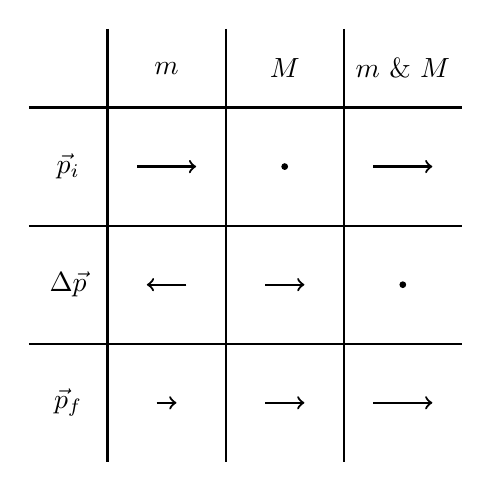
\begin{tikzpicture}
		\MVDRows{MVD}
		\MVDCol{mass}{$m$}{MVD}{0.75}
		\MVec{massinit}{0.75}
		\MVec[180]{massdelt}{0.5}
		\MVec{massfin}{0.25}
		\MVDCol{Mass}{$M$}{mass}{0.75}
		\MDot{Massinit}
		\MVec{Massdelt}{0.5}
		\MVec{Massfin}{0.5}
		\MVDCol{sys}{$m$ \& $M$}{Mass}{0.75}
		\MVec{sysinit}{0.75}
		\MDot{sysdelt}
		\MVec{sysfin}{0.75}
	\end{tikzpicture}
\end{figure}

The momentum conservation equation (choosing right as the positive direction) is
\[
mv = mv_{m} + Mv_{M}.
\]
Since the collision is perfectly elastic, we also have conservation of energy:
\[
\frac{1}{2}mv^{2} = \frac{1}{2}mv_{m}^{2} + \frac{1}{2}Mv_{M}^{2}.
\]
We can use these two equations to solve for both unknown final velocities.

First, let us simplify both expressions by dividing through by $m$ (and multiplying the energy equation by 2):
\begin{align*}
	v & = v_{m} + \frac{M}{m}v_{M}, \\
	v^{2} & = v_{m}^{2} + \frac{M}{m}v_{M}^{2}.
\end{align*}
We can write the first equation as $v_{m} = v - \frac{M}{m}v_{M}$ and substitute it into the second to get
\begin{align*}
	v^{2} & = \left(v - \frac{M}{m}v_{M}\right)^{2} + \frac{M}{m}v_{M}^{2} \\
	v^{2} & = v^{2} - 2\frac{M}{m}vv_{M} + \frac{M^{2}}{m^{2}}v_{M}^{2} + \frac{M}{m}v_{M}^{2} \\
	0 & = - 2\frac{M}{m}vv_{M} + \frac{M^{2}}{m^{2}}v_{M}^{2} + \frac{M}{m}v_{M}^{2}.
\end{align*}
Dividing through by $\frac{M}{m}v_{M}$ gives us
\begin{align*}
	0 & = - 2v + \frac{M}{m}v_{M} + v_{M} \\
	\left(1+\frac{M}{m}\right)v_{M} & = 2v \\
	v_{M} & = \frac{2m}{m+M}v.
\end{align*}
Subsituting this into our simplified momentum expression gives us
\begin{align*}
	v_{m} & = v-\frac{M}{m}\frac{2m}{m+M}v \\
	& = \left(1-\frac{2M}{m+M}\right)v \\
	& = \frac{m-M}{m+M}v.
\end{align*}
}
\Solution{\CollRockSense}{
	
\noindent\textbf{\underline{Sensemaking:}}

If $M \gg m$, then $v_{M}$ approaches zero, as predicted. We also see that $v_{m} \approx -v$, so the small rock reflects back at is original speed.

If $M = m$, then $v_{M}=v$ and $v_{m}=0$, which is the Newton's cradle behavior that we predicted.

We didn't talk about $M \ll m$, but it is interesting. In this case, $v_{m} \approx v$ (the more massive object doesn't slow down after the collision) and $v_{M} \approx 2v$ (the stationary object gets launched forward at twice the massive object's speed). In the reference frame of the massive object, the smaller object is leftbound at speed $v$ and reflects to the right at the same speed, much like the previous special case.
}
%\input{\FileDepth/Activities/Activity_One/Activity_One.tex}
%\input{\FileDepth/Activities/Activity_Two/Activity_Two.tex}

\begin{document}
\begin{TeacherMargin}
\noindent (C) is true, as this condition makes the net impulse on the object zero. If the net force is nonzero, but very weak, or lasting only for a very short while, then we can also say that the impulse is approximately equal.
\end{TeacherMargin}
\begin{PresentSpace}
\begin{center}
	\huge Studio 7: Impulse and Conservation of Momentum \\
	\large (and some energy too)
	\vspace{1cm}
\end{center}
\underline{Warm-Up Activity} \\
Momentum is conserved when\dots
\begin{enumerate}[(A)]
	\item The kinetic energy is zero.
	%\vspace{6pt}
	\item The net external work is zero.
	%\vspace{15pt}
	\item The net force is zero.
	\item There is no change in potential energy.
\end{enumerate}
\end{PresentSpace}
\newpage
\begin{TeacherMargin}
\noindent We want to include the Earth and the spring in our system with the seat and passenger in order to use conservation of energy. If we don't, then we have to go to the trouble  of calculating work done by gravity and the spring. \\

\noindent At $t_{1}$, the person and seat are stationary, and the spring is compressed beneath them. All energy is spring potential energy.
\begin{center}
	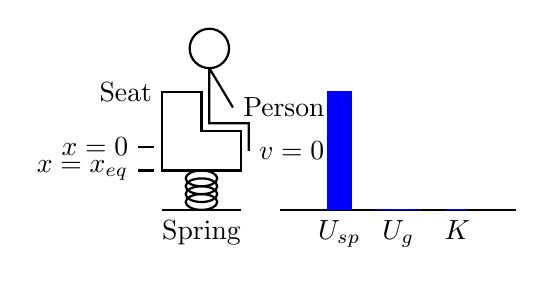
\begin{tikzpicture}
		\begin{scope}
			\draw[thick] (-0.5,0) -- (0,0) node[anchor=north] {Spring} -- (0.5,0);
			\foreach \s in {0,1,2,3}
				\draw[thick] (0,0.1*\s+0.1) circle (0.2 and 0.1);
			\draw[thick,shift={(0,0.5)}] (-0.5,0) -- (-0.5,1)  node[anchor=east] {Seat} -- (0,1) -- (0,0.5) -- (0.5,0.5) -- (0.5,0) -- cycle;
			\draw[thick,shift={(0,0.5)}] (0.6,0.25) node[anchor=west] {$v=0$} -- (0.6,0.6) -- (0.1,0.6) -- (0.1,1.3) arc (270:-90:0.25) -- (0.4,0.8) node[anchor=west] {Person};
			\draw[thick] (-0.6,0.8) -- (-0.8,0.8) node[anchor=east] {$x=0$};
			\draw[thick] (-0.6,0.5) -- (-0.8,0.5) node[anchor=east] {$x=x_{eq}$};
		\end{scope}
		\begin{scope}[shift={(2.5,0)}]
			\draw[thick] (-1.5,0) -- (-0.75,0) node[anchor=north] {$U_{sp}$} -- (0,0) node[anchor=north] {$U_{g}$} -- (0.75,0) node[anchor=north] {$K$} -- (1.5,0);
			\filldraw[blue] (-0.9,0) rectangle (-0.6,1.5);
			\filldraw[blue] (-0.3,0) rectangle (0.3,0);
			\filldraw[blue] (0.6,0) rectangle (0.9,0);
		\end{scope}
	\end{tikzpicture}
\end{center}
Here, I define the amount by which the spring was compressed as $x_{c}$, and I set $x=0$ at the top of the spring. \\

\noindent At $t_{2}$, the spring is at its equilibrium length, and the person and seat have been lifted up slightly and now have some speed. The spring potential energy has all been transformed into kinetic energy and a little bit of gravitational potential energy.
\begin{center}
	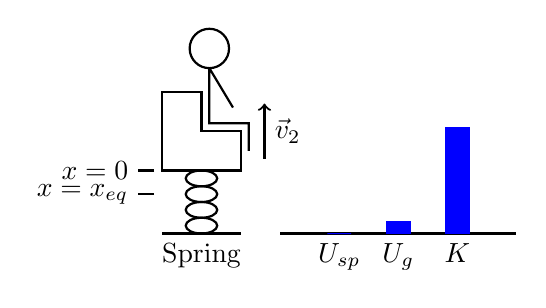
\begin{tikzpicture}
		\begin{scope}
			\draw[thick] (-0.5,0) -- (0,0) node[anchor=north] {Spring} -- (0.5,0);
			\foreach \s in {0,1,2,3}
			\draw[thick] (0,0.2*\s+0.1) circle (0.2 and 0.1);
			\draw[thick,shift={(0,0.8)}] (-0.5,0) -- (-0.5,1) -- (0,1) -- (0,0.5) -- (0.5,0.5) -- (0.5,0) -- cycle;
			\draw[thick,shift={(0,0.8)}] (0.6,0.25) -- (0.6,0.6) -- (0.1,0.6) -- (0.1,1.3) arc (270:-90:0.25) -- (0.4,0.8);
			\draw[thick,->] (0.8,0.95) -- (0.8,1.3) node[anchor=west] {$\vec{v}_{2}$} -- (0.8,1.65);
			\draw[thick] (-0.6,0.8) -- (-0.8,0.8) node[anchor=east] {$x=0$};
			\draw[thick] (-0.6,0.5) -- (-0.8,0.5) node[anchor=east] {$x=x_{eq}$};
		\end{scope}
		\begin{scope}[shift={(2.5,0)}]
			\draw[thick] (-1.5,0) -- (-0.75,0) node[anchor=north] {$U_{sp}$} -- (0,0) node[anchor=north] {$U_{g}$} -- (0.75,0) node[anchor=north] {$K$} -- (1.5,0);
			\filldraw[blue] (-0.9,0) rectangle (-0.6,0);
			\filldraw[blue] (-0.15,0) rectangle (0.15,0.15);
			\filldraw[blue] (0.6,0) rectangle (0.9,1.35);
		\end{scope}
	\end{tikzpicture}
\end{center}
I use the label $v_{2}$ fr the speed at this moment. It is not $v_{max}$, which would actually happen before the spring reaches equilibrium. \\

At $t_{3}$, the person and seat stop momentarily at their maximum height. The kinetic energy has all been transformed into gravitational potential energy.
\begin{center}
	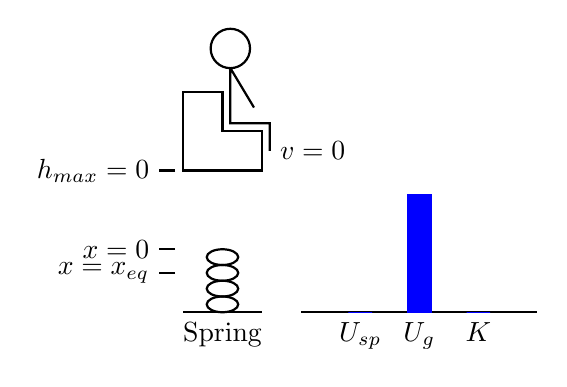
\begin{tikzpicture}
		\begin{scope}
			\draw[thick] (-0.5,0) -- (0,0) node[anchor=north] {Spring} -- (0.5,0);
			\foreach \s in {0,1,2,3}
			\draw[thick] (0,0.2*\s+0.1) circle (0.2 and 0.1);
			\draw[thick,shift={(0,1.8)}] (-0.5,0) -- (-0.5,1) -- (0,1) -- (0,0.5) -- (0.5,0.5) -- (0.5,0) -- cycle;
			\draw[thick,shift={(0,1.8)}] (0.6,0.25) node[anchor=west] {$v=0$} -- (0.6,0.6) -- (0.1,0.6) -- (0.1,1.3) arc (270:-90:0.25) -- (0.4,0.8);
			\draw[thick] (-0.6,1.8) -- (-0.8,1.8) node[anchor=east] {$h_{max}=0$};
			\draw[thick] (-0.6,0.8) -- (-0.8,0.8) node[anchor=east] {$x=0$};
			\draw[thick] (-0.6,0.5) -- (-0.8,0.5) node[anchor=east] {$x=x_{eq}$};
		\end{scope}
		\begin{scope}[shift={(2.5,0)}]
			\draw[thick] (-1.5,0) -- (-0.75,0) node[anchor=north] {$U_{sp}$} -- (0,0) node[anchor=north] {$U_{g}$} -- (0.75,0) node[anchor=north] {$K$} -- (1.5,0);
			\filldraw[blue] (-0.9,0) rectangle (-0.6,0);
			\filldraw[blue] (-0.15,0) rectangle (0.15,1.5);
			\filldraw[blue] (0.6,0) rectangle (0.9,0);
		\end{scope}
	\end{tikzpicture}
\end{center}
\begin{center}
	\begin{tabular}{c||c|c|c||c}
		& $U_{sp}$ & $U_{g}$ & $K$ & $E_{\text{total}}$ \\ \hline
		$t_{1}$ & $\frac{1}{2}kx_{c}^{2}$ & 0 & 0 & $\frac{1}{2}kx_{c}^{2}$ \\ \hline
		$t_{2}$ & 0 & $mgx_{c}$ & $\frac{1}{2}mv_{2}^{2}$ & $mgx_{c}+\frac{1}{2}mv_{2}^{2}$ \\ \hline
		$t_{3}$ & 0 & $mgh_{max}$ & 0 & $mgh_{max}$
	\end{tabular}
\end{center}
\end{TeacherMargin}
\begin{PresentSpace}
\vspace{-10pt}
\section*{S7-1: Ejector Seat}
\vspace{-10pt}
\begin{itemize}
	\large
	\item A stationary stunt car driver has an ejector seat that rests on a compressed vertical spring.
	\item When the spring is released, the seat with its passenger is launched out of the car and into the air.
	\begin{itemize}
		\normalsize
		\item Explain why you might want to include the Earth and the spring in your system.
	\end{itemize}
	\item Consider three instants in time: (1) just before the seat is released, (2) when the spring is at equilibrium, and (3) the person reaches maximum height.
	\begin{itemize}
		\normalsize
		\item Write a qualitative description of how the energy of the system transforms through these three instants.
	\end{itemize}
	\item For each instant:
	\begin{itemize}
		\normalsize
		\item Draw a physical diagram.
		\item Construct an energy bar chart.
		\item Write each energy symbolically.
	\end{itemize}
	\item How high does the person go?
	\item What is the person's speed when the ejector seat leaves the spring?
	\begin{itemize}
		\item Don't forget to make sense of your answers!
	\end{itemize}
\end{itemize}
\end{PresentSpace}
\newpage
\begin{TeacherMargin}
\begin{center}
	\begin{tabular}{c||c|c|c||c}
		& $U_{sp}$ & $U_{g}$ & $K$ & $E_{\text{total}}$ \\ \hline
		$t_{1}$ & $\frac{1}{2}kx_{c}^{2}$ & 0 & 0 & $\frac{1}{2}kx_{c}^{2}$ \\ \hline
		$t_{2}$ & 0 & $mgx_{c}$ & $\frac{1}{2}mv_{2}^{2}$ & $mgx_{c}+\frac{1}{2}mv_{2}^{2}$ \\ \hline
		$t_{3}$ & 0 & $mgh_{max}$ & 0 & $mgh_{max}$
	\end{tabular}
\end{center}
If there is no external work between any two times, then the $E_{\text{total}}$ entries for those times are equal!
%\begin{multicols}{2}
\begin{align*}
	E_{\text{total,1}} = E_{\text{total,3}} \implies \frac{1}{2}kx_{c}^{2} = mgh_{max} \implies h_{max}=\frac{kx_{c}^{2}}{2mg}
\end{align*}
\begin{align*}
	E_{\text{total,1}} = E_{\text{total,2}} \implies
	\frac{1}{2}kx_{c}^{2} = mghx_{c} + \frac{1}{2}mv_{2}^{2} & \implies
	\left(\frac{k}{m}x_{c}-2g\right)x_{c} = v_{2}^{2} \\
	& \implies
	v_{2} = \sqrt{\left(\sqrt{\frac{k}{m}}-2g\right)x_{c}}
\end{align*}
%\end{multicols}
\vspace{-1.8cm} \\
\textbf{Sensemaking} \\
\begin{itemize}
	\item $h_{max}=\frac{kx_{c}^{3}}{2mg}$
	\begin{itemize}
		\item Unit Check: $[h_{max}]=\frac{[k][x_{c}]^{2}}{[mg]} = \frac{\frac{\text{N}}{\text{m}}\cdot\text{m}^{2}}{\text{N}} = m$
		\item Covariation
		\begin{itemize}
			\item $k$ increases or $x_{c}$ increases $\implies$ $h_{max}$ increases. \\
			A stiffer spring, (higher $k$) stores more energy for the same compression, and a more compressed spring (higher $x_{c}$) stores more energy. Imparting more kinetic energy to the seat and person will allow them to go higher.
			\item $m$ increases or $g$ increases $\implies$ $h_{max}$ decreases. \\
			A more massive object will store more gravitational potential energy in less of an elevation change, as would an object in stronger gravity. As such, the object would transform its kinetic energy entirely at a smaller maximum height.
		\end{itemize}
	\end{itemize}
	\item $v_{2}=\sqrt{\left(\frac{k}{m}x_{c}-2g\right)x_{c}}$
	\begin{itemize}
		\item Unit Check:
		\begin{align*}
		[v_{2}] & = \sqrt{\left(\frac{[k]}{[m]}[x_{c}]-[g]\right)[x_{c}]} = \sqrt{\left(\frac{\text{N}/\text{m}}{\text{kg}}\cdot\text{m}-\frac{\text{m}}{\text{s}^{2}}\right)\cdot\text{m}} \\
		& = \sqrt{\frac{\text{N}\cdot\text{m}}{\text{kg}}-\frac{\text{m}^{2}}{\text{s}^{2}}} = \sqrt{\frac{\text{m}^{2}}{\text{s}^{2}}-\frac{\text{m}^{2}}{\text{s}^{2}}} = \frac{\text{m}}{\text{s}}
		\end{align*}
		\item Special Cases
		\begin{itemize}
			\item What if $\frac{k}{m}x_{c} = 2g$? \\
			The equation would say $v_{2}=0$, so the seat does not leave the spring. Rearranging, we can see that $x_{c} = \frac{2mg}{k}$, and when we plug this into our equation for $h_{max}$, we get $h_{max}=x_{c}$, so our equations are consistent with each other.
			\item What if $\frac{k}{m}x_{c} < 2g$? \\
			Then $v_{2}$ is not real (we are talking about the square root of an imaginary number). \\
			Physically, if $x_{c} < \frac{2mg}{k}$, then the spring never fully decompresses, and $v_{2}$ is defined based on the assumption that it does, so it makes sense that we would get an invalid answer.
		\end{itemize}
	\end{itemize}
\end{itemize}
\end{TeacherMargin}
\begin{PresentSpace}
\vspace{-10pt}
\section*{S7-1: Ejector Seat}
\vspace{-10pt}
\begin{itemize}
	\large
	\item A stationary stunt car driver has an ejector seat that rests on a compressed vertical spring.
	\item When the spring is released, the seat with its passenger is launched out of the car and into the air.
	\begin{itemize}
		\normalsize
		\item Explain why you might want to include the Earth and the spring in your system.
	\end{itemize}
	\item Consider three instants in time: (1) just before the seat is released, (2) when the spring is at equilibrium, and (3) the person reaches maximum height.
	\begin{itemize}
		\normalsize
		\item Write a qualitative description of how the energy of the system transforms through these three instants.
	\end{itemize}
	\item For each instant:
	\begin{itemize}
		\normalsize
		\item Draw a physical diagram.
		\item Construct an energy bar chart.
		\item Write each energy symbolically.
	\end{itemize}
	\item How high does the person go?
	\item What is the person's speed when the ejector seat leaves the spring?
	\begin{itemize}
		\item Don't forget to make sense of your answers!
	\end{itemize}
\end{itemize}
\end{PresentSpace}
\newpage
\begin{TeacherMargin}

\end{TeacherMargin}
\begin{PresentSpace}
\vspace{-10pt}
\section*{Impulse and Momentum}
\vspace{-5pt}
We rewrote Newton's 2nd law in a new way, which we will call the impulse-momentum theorem.
\begin{align*}
	\text{Impulse} & = \text{Change in Momentum} \\
	\vec{J}_{net} & = \Delta\vec{p} \\
	\int_{t_{i}}^{t_{f}}\vec{F}^{net}dt & = m\vec{v}_{f}-m\vec{v}_{i}
\end{align*}
\end{PresentSpace}
\newpage
\begin{TeacherMargin}

\end{TeacherMargin}
\begin{PresentSpace}
\vspace{-10pt}
\section*{A Deeper Model for Interactions}
\vspace{-10pt}
\begin{itemize}
	\item Quantities
	\begin{itemize}
		\item Energy \qquad \qquad \qquad \quad \ \ $E$
		\item Work \qquad \qquad \qquad \quad \ \ \ \ $W = \int_{r_{i}}^{r_{f}}\vec{F}\cdot d\vec{r}$
		\item Kinetic Energy \qquad \qquad $K=\frac{1}{2}mv^{2}$
		\item Potential Energy \qquad \quad \ $U=$ depends on interaction \\
		You have to tell everyone where zero $PE$ is!
		\begin{itemize}
			\item Gravity \qquad $U_{g} = mgy$
			\item Spring \qquad \ $U_{sp} = \frac{1}{2}kx^{2}$
		\end{itemize}
		\item Momentum \qquad \qquad \qquad $\vec{p}=m\vec{v}$
		\item Impulse \qquad \qquad \quad \quad \ \ $\vec{J}_{net}=\int_{t_{i}}^{t_{f}}\vec{F}^{net}dt$
	\end{itemize}
	\item Laws
	\begin{itemize}
		\item Work-energy theorem \qquad $W_{\text{net,ext}} = \Delta E_{\text{total}}$
		\item Impulse-momentum theorem \qquad $\vec{J}_{net} = \Delta\vec{p}$
	\end{itemize}
\end{itemize}
\end{PresentSpace}
\newpage
\begin{TeacherMargin}
\begin{center}
	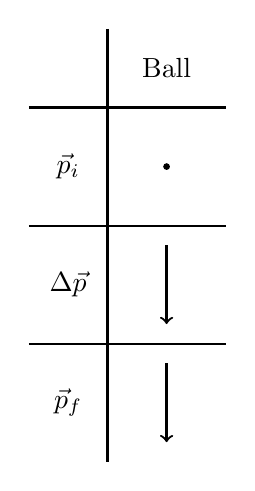
\begin{tikzpicture}
		\MVDRows[1.5]{B}
		\MVDCol{DropB}{Ball}{B}
		\MDot{DropBinit}
		\MVec[270]{DropBdelt}{1}
		\MVec[270]{DropBfin}{1}
	\end{tikzpicture}
\end{center}
This problem gives us the simple momentum vector diagram above. We know that $\vec{F}^{net} =\vec{F}^{g}$ during the fall, so the impulse is
\begin{align*}
	\vec{J}_{net} = \int_{t_{i}}^{t_{f}}\vec{F}^{net}dt & = m\vec{v}_{f} - m\vec{v}_{i} \\
	-mg\Delta t & = mv_{f} \\
	-g\Delta t & = v_{f}.
\end{align*}
Plugging in numbers ($g\approx 10$ m/s$^{2}$ and $\Delta t = 0.5$ s) gives us $v_{f} = -5\text{m}/\text{s}$
\end{TeacherMargin}
\begin{PresentSpace}
\vspace{-10pt}
\section*{S7-2: The Ball and the Ground I}
\vspace{-10pt}
\begin{itemize}
	\item You drop a 0.05 kg tennis ball from rest and it takes 0.5 s to hit the ground.
	\item Use the impulse-momentum theorem to find the velocity of the ball just before impact with the ground.
\end{itemize}
\end{PresentSpace}
\newpage
\begin{TeacherMargin}
\begin{center}
	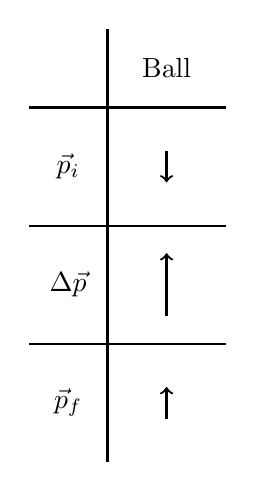
\begin{tikzpicture}
		\MVDRows[1.5]{B}
		\MVDCol{DropB}{Ball}{B}
		\MVec[270]{DropBinit}{0.4}
		\MVec[90]{DropBdelt}{0.8}
		\MVec[90]{DropBfin}{0.4}
	\end{tikzpicture}
\end{center}
Let the velocities before and after the bounce be $\vec{v}_{i} = -5\text{ m}/\text{s}\hat{y}$ and $\vec{v}_{f} = 5\text{ m}/\text{s}\hat{y}$. The change in momentum is
\[
\Delta\vec{p} = m\vec{v}_{f} - m\vec{v_{i}} = m \left(\vec{v}_{f} - m\vec{v_{i}}\right) = (0.05\text{ kg})(5\text{ m}/\text{s} - (-5\text{ m}/\text{s}))\hat{y} = 0.5 \text{kg m/s}^{2}\hat{y}.
\]
We can simplify the impulse integral by writing it in terms of the net force:
\[
\int_{t_{i}}^{t_{f}}\vec{F}^{net}dt = \vec{F}^{net}_{avg}\Delta t.
\]
As such,
\[
\vec{F}^{net}_{avg}\Delta t = \Delta\vec{p} \implies \vec{F}^{net}_{avg} = \frac{m}{\Delta t}\left(\vec{v}_{f}-\vec{v}_{i}\right).
\]
With numbers, this becomes
\[
\vec{F}^{net}_{avg} = \frac{0.05\text{ kg}}{0.01\text{ s}}\left(5\text{ m}/\text{s}-(-5\text{ m}/\text{s})\right)\hat{y} = (50\text{ N})\hat{y}.
\]
If we subtract off the force of gravity (-0.5 N $\hat{y}$), we can find out the average normal force (50.5 N).
\end{TeacherMargin}
\begin{PresentSpace}
\vspace{-10pt}
\section*{S7-2: The Ball and the Ground II}
\vspace{-10pt}
\begin{itemize}
	\item  You drop a 0.05 kg tennis ball from rest and it takes 0.5 s to hit the ground.
	\item The tennis ball rebounds from the ground with the same speed as impact. The collision takes 0.01 s.
	\item Find the average net force on the tennis ball.
\end{itemize}
\end{PresentSpace}
\newpage
\begin{TeacherMargin}

\end{TeacherMargin}
\begin{PresentSpace}
\vspace{-10pt}
\section*{Conservation of Momentum}
\vspace{-5pt}
If the net force on a system is zero, then the impulse is zero.
\begin{align*}
	\vec{J} & = \Delta\vec{p} \\
	\vec{0} & = \Delta\vec{p}
\end{align*}
Under this condition, we say that the momentum of the system is \textit{conserved}---it does not change!
\end{PresentSpace}
\newpage
\begin{TeacherMargin}
\CollRockConsSol
\CollRocksSpecSol
%\CollRockCalc
%\CollRockSense
\end{TeacherMargin}
\begin{PresentSpace}
\vspace{-10pt}
\section*{S7-3: Two Rocks Collide}
\vspace{-10pt}
\begin{itemize}
	\item A small rock (mass $m$) is moving to the right on a frictionless table with speed $v$.
	\item It hits a second rock (mass $M$) that is initially at rest on the table. The rocks do not stick together.
	\begin{itemize}
		\item Is momentum conserved? For what system?
		\item Is energy conserved? For what system?
	\end{itemize}
	\item Our goal is to find the final speed of each rock, but don't try to solve it yet.
	\begin{itemize}
		\item Instead, what special cases do you want to think about for this situation? What makes these special cases easier to think about than the general problem?
	\end{itemize}
\end{itemize}
\end{PresentSpace}
\newpage
\begin{TeacherMargin}
%\CollRockConsSol
%\CollRocksSpecSol
\begin{multicols}{2}
\CollRockCalc
\CollRockSense
\end{multicols}
\end{TeacherMargin}
\begin{PresentSpace}
\vspace{-10pt}
\section*{S7-3: Two Rocks Collide}
\vspace{-10pt}
\begin{itemize}
	\item A small rock (mass $m$) is moving to the right on a frictionless table with speed $v$.
	\item It hits a second rock (mass $M$) that is initially at rest on the table. The rocks do not stick together.
	\begin{itemize}
		\item Is momentum conserved? For what system?
		\item Is energy conserved? For what system?
	\end{itemize}
	\item Our goal is to find the final speed of each rock, but don't try to solve it yet.
	\begin{itemize}
		\item Instead, what special cases do you want to think about for this situation? What makes these special cases easier to think about than the general problem?
	\end{itemize}
\end{itemize}
\end{PresentSpace}
\newpage
\begin{TeacherMargin}

\end{TeacherMargin}
\begin{PresentSpace}
\vspace{-10pt}
\section*{Energy and Collisions}
\vspace{-10pt}
\begin{itemize}
	\item Collisions where kinetic energy is conserved are known as \textit{elastic collisions}.
	\item Collisions where the energy of the system decreases are known as \textit{inelastic collisions}.
	\begin{itemize}
		\item When two things stick together, this is a \textit{perfectly inelastic collision}.
	\end{itemize}
	\item Collisions where the energy of the system increases are known as \textit{superelastic collisions}.
	\begin{itemize}
		\item Think explosions.
	\end{itemize}
\end{itemize}
\end{PresentSpace}
\newpage
\begin{TeacherMargin}

\end{TeacherMargin}
\begin{PresentSpace}
\section*{Main Ideas}
\begin{itemize}
	\item Momentum and impulse are useful quantities for solving dynamics problems.
	\item The impulse is always equal to the change in momentum for a system.
	\item When the impulse is zero (because the net force is zero), the momentum of the system is constant---it is \textit{conserved}.
\end{itemize}
\end{PresentSpace}
\end{document}